
En la figura de este problema se ilustra un triángulo rectángulo \textit{ABC} situado frente a un espejo cóncavo, de centro \textit{C} y distancia focal igual a 6,0 cm. Sabiendo que \textit{AB} = 8,0 cm y \textit{AC} = 60 cm, determine el área de la imagen del triángulo \textit{ABC}, proporcionada por el espejo.
\begin{figure}[h!]
    \centering
    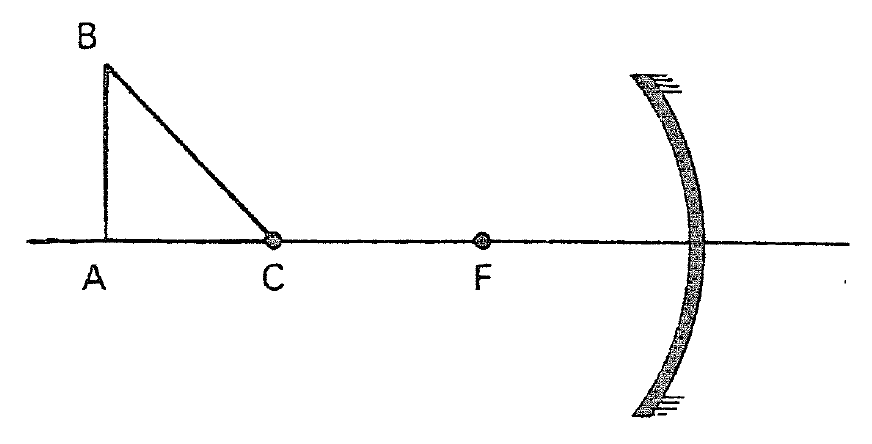
\includegraphics[scale=0.4]{enunciados/alvarenga_p655_10.png}
    \caption{Alvarenga p. 655 - Problema complementario 10}
\end{figure}